\documentclass{article}

% if you need to pass options to natbib, use, e.g.:
%     \PassOptionsToPackage{numbers, compress}{natbib}
% before loading neurips_2025

% The authors should use one of these tracks.
% Before accepting by the NeurIPS conference, select one of the options below.
% 0. "default" for submission
 % \usepackage{neurips_2025}
% the "default" option is equal to the "main" option, which is used for the Main Track with double-blind reviewing.
% 1. "main" option is used for the Main Track
 % \usepackage[main]{neurips_2025}
% 2. "position" option is used for the Position Paper Track
%  \usepackage[position]{neurips_2025}
% 3. "dandb" option is used for the Datasets & Benchmarks Track
 % \usepackage[dandb]{neurips_2025}
% 4. "creativeai" option is used for the Creative AI Track
%  \usepackage[creativeai]{neurips_2025}
% 5. "sglblindworkshop" option is used for the Workshop with single-blind reviewing
 % \usepackage[sglblindworkshop]{neurips_2025}
% 6. "dblblindworkshop" option is used for the Workshop with double-blind reviewing
%  \usepackage[dblblindworkshop]{neurips_2025}

% After being accepted, the authors should add "final" behind the track to compile a camera-ready version.
% 1. Main Track
 \usepackage[main, final]{neurips_2025}
% 2. Position Paper Track
%  \usepackage[position, final]{neurips_2025}
% 3. Datasets & Benchmarks Track
 % \usepackage[dandb, final]{neurips_2025}
% 4. Creative AI Track
%  \usepackage[creativeai, final]{neurips_2025}
% 5. Workshop with single-blind reviewing
%  \usepackage[sglblindworkshop, final]{neurips_2025}
% 6. Workshop with double-blind reviewing
%  \usepackage[dblblindworkshop, final]{neurips_2025}
% Note. For the workshop paper template, both \title{} and \workshoptitle{} are required, with the former indicating the paper title shown in the title and the latter indicating the workshop title displayed in the footnote.
% For workshops (5., 6.), the authors should add the name of the workshop, "\workshoptitle" command is used to set the workshop title.
% \workshoptitle{WORKSHOP TITLE}

% "preprint" option is used for arXiv or other preprint submissions
 % \usepackage[preprint]{neurips_2025}

% to avoid loading the natbib package, add option nonatbib:
%    \usepackage[nonatbib]{neurips_2025}

\usepackage[utf8]{inputenc} % allow utf-8 input
\usepackage[T1]{fontenc}    % use 8-bit T1 fonts
\usepackage{hyperref}       % hyperlinks
\usepackage{url}            % simple URL typesetting
\usepackage{booktabs}       % professional-quality tables
\usepackage{amsfonts}       % blackboard math symbols
\usepackage{nicefrac}       % compact symbols for 1/2, etc.
\usepackage{microtype}      % microtypography
\usepackage{xcolor}         % colors
\usepackage{amsmath}
% \usepackage[numbers]{natbib} % or authoryear
\usepackage[most]{tcolorbox}
\tcbset{
  custombox/.style={
    width=\linewidth,
    top=10pt,
    bottom=6pt,
    colback=gray!5!white,
    colframe=darkgray,
    colbacktitle=darkgray,
    enhanced,
    center,
    attach boxed title to top left={yshift=-0.12in,xshift=0.2in},
    boxed title style={
      boxrule=0pt,
      colframe=white,
      rounded corners,
      interior style={color=black}
    },
  }
}
\newtcolorbox{CustomBox}[2][]{custombox,title=#2,#1}
\definecolor{darkgray}{rgb}{0.25,0.25,0.25}

% Note. For the workshop paper template, both \title{} and \workshoptitle{} are required, with the former indicating the paper title shown in the title and the latter indicating the workshop title displayed in the footnote. 
\title{A Theoretical Perspective on Cognitive Security}

% The \author macro works with any number of authors. There are two commands
% used to separate the names and addresses of multiple authors: \And and \AND.
%
% Using \And between authors leaves it to LaTeX to determine where to break the
% lines. Using \AND forces a line break at that point. So, if LaTeX puts 3 of 4
% authors names on the first line, and the last on the second line, try using
% \AND instead of \And before the third author name.


\author{%
 Batu El\\
  Stanford University\\
  \texttt{batuel@stanford.edu} \\
  % examples of more authors
  % \And
  % Coauthor \\
  % Affiliation \\
  % Address \\
  % \texttt{email} \\
  % \AND
  % Coauthor \\
  % Affiliation \\
  % Address \\
  % \texttt{email} \\
  % \And
  % Coauthor \\
  % Affiliation \\
  % Address \\
  % \texttt{email} \\
  % \And
  % Coauthor \\
  % Affiliation \\
  % Address \\
  % \texttt{email} \\
}


\begin{document}

\maketitle
% \begin{figure}[ht]
%     \centering
%     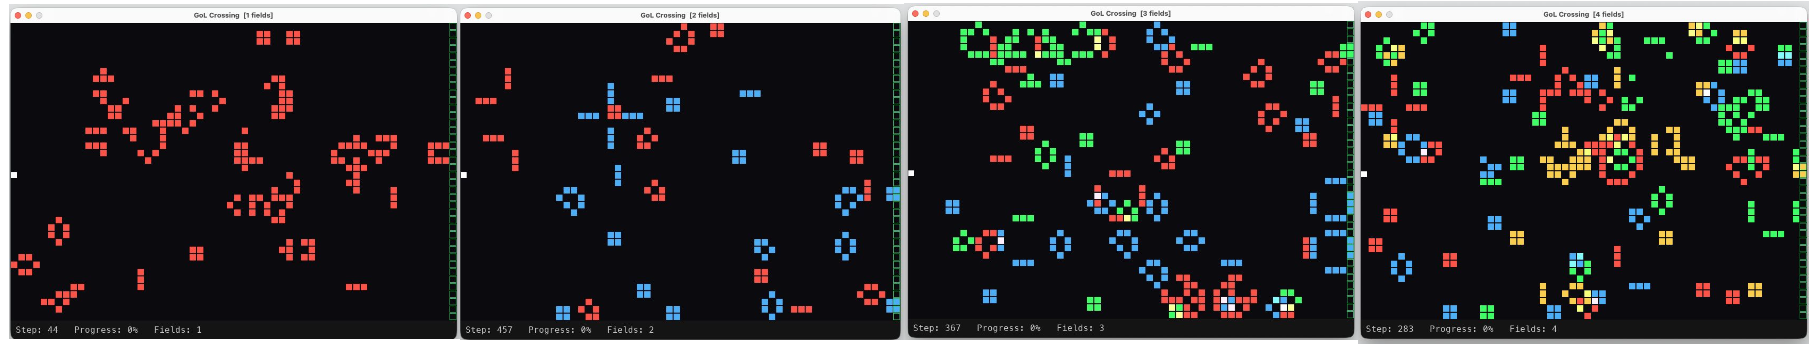
\includegraphics[width=0.99\linewidth]{Figures/Figure1.png}
%     \caption{\textit{Example game environment setup showing the Frame Crossing Game at increasing complexity levels (1–4 fields).} The agent (white cell, left edge) must navigate across the 96×96 grid to the right edge while avoiding live cells, whose evolution follows Conway's Game of Life rules. Each additional field introduces an independent population of cells (shown in distinct colors), increasing environment complexity and obstacle density.}
%     \label{fig:gol_panels}
% \end{figure}
\begin{abstract}
\input{Sections/0_abstract}
\end{abstract}

\section{Prelude}

Today, recommender algorithms are powerful enough to keep us scrolling for hours. At their core, they are a cognitive process: they map inputs (a person's history, preferences, and behavior) to an output (the next piece of content that person will see). Two major shifts are happening which will make this process far more potent.

\textit{The input space is expanding.} The signals feeding these algorithms are growing richer by the day. We have moved from expressed preferences (what you liked, what your friends liked, how long you watched a video, what you commented) to physiological responses: how your pupils dilated or your heart rate spiked when you saw something. Language model apps record conversations and construct detailed psychological profiles. Wearables and smart glasses collect continuous biometric data. And increasingly, AI is becoming a therapist, a confidant, a life coach—one that knows every vulnerable detail about you.

\textit{The output space is becoming generative.} On the other side, what algorithms can serve is no longer limited to selecting from existing content. Generative AI allows systems to produce bespoke videos, images, narratives, and experiences. This content is sculpted specifically for an individual, in real time.

\textit{Where is this heading?} With richer inputs and more flexible outputs, the accuracy of these systems will only improve. At the lower bound, they will simply be more of what they already are—more precise, more addictive, more relentless. At the upper bound, they converge on something like the Matrix: hyper-personalized, immersive, physiologically optimized realities. The urgent question, then, is not whether this world arrives, but how it should be governed.

\textit{But can this be made useful?} The same machinery of engagement need not only serve distraction or profit. If these systems can hold human attention so effectively, they could, in principle, direct it toward something worthwhile—channeling engagement into socially valuable tasks: scientific discovery through citizen science, democratic deliberation, collective problem-solving, education, or caregiving. The most powerful attention engine ever built could be a force for coordination rather than mere consumption.



\section{Introduction}
Cognitive security is the \textit{protection of cognitive processes from hazardous influence}.

\textbf{\textit{Cognitive Process.}} A cognitive process is the mechanism by which an agent (biological or artificial) transforms inputs into outputs. It has three components:

(a) \textit{Policy} captures the agent's dispositions: the accumulated knowledge, beliefs, values, and learned associations it carries into any given situation.\\
(b) \textit{State} captures the agent's immediate experience: the particular context it currently finds itself in.\\
(c) \textit{Action} captures the agent's output: the belief, judgment, or behavior it produces in response to its state.

The cognitive process uses \textit{policy} to map \textit{state} to \textit{action}.

\textit{This distinction matters because influence can target any of the three components. Influence that operates on state is transient: remove the stimulus and the agent reverts to its prior behavior. Influence that gradually reshapes policy is persistent: it alters how the agent responds even long after the stimulus is gone. Influence that operates on action is direct: it bypasses the cognitive process entirely, constraining or compelling what the agent can do regardless of what it believes or intends, such as in the case of physical coercion or censorship.}




\textbf{\textit{Hazardous Influence.}} Hazardous influence means any act of influence that is exercised with intent to, or that carries a reasonable potential to:

(a) induce or facilitate conduct that is unlawful under applicable law;\\
(b) cause harm (physical, psychological, financial, or reputational) to the person influenced; or\\
(c) impair the integrity of the public institutions that rely on the faithful aggregation of individual preferences, such as democratic processes and free markets.

Influence that neither satisfies nor carries a reasonable potential to satisfy any of (a), (b), or (c) is non-hazardous influence.



\section{Setup}

we want to implement a mapping from $s \rightarrow a_{\text{target}}$. 

Here, query can be a statement or a situation. a can be an answer or an action.

The person processes

$f_{\theta}(c, s) = a$

The attacker can either choose $c$, such that 




\textbf{Attack.}
Context attack. 



Parameter attack.

- what can be done for the parameter attacks to last longer / to be more effective?

- how this relates to the original learning problem?

- how this relates to continual learning setup?

- how this relates to the curriculum learning setup?

\textbf{Defense.}
Context defense. 

- how this relates to safety finetuning?



Parameter defense.

- how this relates to making the models more resiliaent against unsafe fine tuning practices.

- how 

\label{sec:intro}
\input{Sections/1_introduction}
\section{Background}
\label{sec:background}
\input{Sections/2_background}
\section{Setup}
\label{sec:setup}
\section{Formal Models of Influence and Cognitive Process }
\label{appendix:formal-model}
 We model cognition ( human or machine) as a parameterized function that maps inputs to outputs.
 
\begin{definition}[Cognitive Process]
Let $F_\theta$ denote a \emph{cognitive process} parameterized by $\theta \in \Theta$. The process maps an input to an output:
\begin{equation}
    F_\theta(\mathbf{x}) = \mathbf{y},
\end{equation}
where the input $\mathbf{x} = (c, q)$ consists of a \emph{context} $c$ and a \emph{question} $q$, and the output $\mathbf{y} = a$ is the agent's \emph{answer} to the question.
\end{definition}
 
\textit{Generality across agents.} This formulation applies uniformly to both human and machine cognition. Different individuals correspond to different parameter vectors $\theta_{\mathrm{human}}^{(i)}$, and different models correspond to different parameter vectors $\theta_{\mathrm{model}}^{(j)}$. The parameter $\theta$ encodes the totality of an agent's prior knowledge, biases, and learned associations that determine how it processes inputs.
 
\section{First-Order Influence (Context Manipulation)}
 
First-order influence operates by modifying the \emph{input} to a cognitive process while leaving its parameters fixed. The attacker seeks a context that, when prepended to the input, shifts the agent's response from $a$ to a target response $a'$.
 
\paragraph{Initial survey.} Under a baseline context $c_0$, the agent responds:
\begin{equation}
    F_\theta(c_0,\, q) = a.
\end{equation}
 
\paragraph{Attacker's objective.} The attacker solves for an adversarial context $c_1^*$:
\begin{equation}
    c_1^* = \arg\min_{c_1} \; \mathcal{L}\!\bigl(F_\theta(c_1,\, q),\; a'\bigr),
\end{equation}
where $\mathcal{L}$ is a loss measuring the discrepancy between the agent's output and the attacker's target $a'$.
 
\paragraph{Final survey.} After the attack, the agent responds:
\begin{equation}
    F_\theta(c_1^*,\, q) = a'.
\end{equation}
 
The parameters $\theta$ remain unchanged throughout first-order influence. The attack surface is entirely the input space. This is analogous to prompt injection or in-context persuasion: the agent's ``mind'' is unaltered, but its behavior is redirected by manipulating what it sees.
 
\section{Second-Order Influence (Parameter Manipulation)}
 
Second-order influence operates by modifying the \emph{parameters} of the cognitive process. The attacker crafts training conditions that, when processed by a learning algorithm, update $\theta$ so that the agent's response changes, even when the original context is restored.
 
\subsection{Learning Algorithm}
 
\begin{definition}[Learning Algorithm]
Let $\Phi$ denote a \emph{learning algorithm} that updates parameters given a batch of training data:
\begin{equation}
    \Phi(\theta_k,\, B) = \theta_{k+1}.
\end{equation}
\end{definition}
 
\begin{definition}[Batch]
A \emph{batch} $B$ is an ordered list of \emph{sub-batches}:
\begin{equation}
    B = [B_1, B_2, \ldots, B_T],
\end{equation}
where each sub-batch $B_t$ is a set of experience triples:
\begin{equation}
    B_t = \bigl\{(x_i,\, y_i,\, r_i)\bigr\}_{i=1}^{n_t},
\end{equation}
with $x_i$ an input, $y_i$ an output, and $r_i \in \mathbb{R}$ a reward signal.
\end{definition}
 
Crucially, the output $y_i$ in each experience triple is \emph{generated by the agent itself}: $y_i = F_{\theta_k}(x_i)$. The attacker controls the inputs $x_i$ and the reward signals $r_i$, but the outputs are determined by the agent's current parameters. A sub-batch is therefore fully specified by the attacker's choices and the agent's responses:
\begin{equation}
    B_t = \bigl\{(x_i,\, F_{\theta_k}(x_i),\, r_i)\bigr\}_{i=1}^{n_t}.
\end{equation}
 
The learning algorithm $\Phi$ subsumes a broad class of update rules. For instance, when $\Phi$ is gradient descent on a loss $\ell$, each sub-batch update takes the form:
\begin{equation}
    \theta_{k+1} = \theta_k - \eta \, \frac{1}{|B_t|} \sum_{(x,y,r) \in B_t} \nabla_\theta \, \ell(\theta_k;\, x, y, r),
\end{equation}
where $\eta > 0$ is the learning rate. In the human setting, $\Phi$ represents the (possibly implicit) process by which lived experiences update an individual's beliefs and dispositions over time. For example, repeated exposure to a particular narrative (batch) may gradually shift one's priors (parameters).
 
\subsection{Attacker's Objective}
 
The attacker controls the \emph{environment}---the inputs presented to the agent and the reward signals delivered in response---but not the agent's outputs, which are generated by the agent's own cognitive process. Formally, the attacker selects a set of input--reward pairs $\mathcal{S} = \{(x_i, r_i)\}_{i=1}^{n}$. The resulting batch is then determined jointly by the attacker's choices and the agent's behavior:
\begin{equation}
    B(\mathcal{S},\, \theta_k) = \bigl\{(x_i,\, F_{\theta_k}(x_i),\, r_i)\bigr\}_{i=1}^{n}.
\end{equation}
 
\paragraph{Initial survey.} Under the current parameters $\theta_k$ and baseline context $c_0$:
\begin{equation}
    F_{\theta_k}(c_0,\, q) = a.
\end{equation}
 
\paragraph{Attacker's objective.} The attacker solves for an adversarial set of input--reward pairs $\mathcal{S}^*$:
\begin{equation}
    \mathcal{S}^* = \arg\min_{\mathcal{S}} \; \mathcal{L}\!\bigl(F_{\Phi(\theta_k,\, B(\mathcal{S},\, \theta_k))}(c_0,\, q),\; a'\bigr).
\end{equation}
That is, the attacker selects inputs and reward signals such that, after the agent generates its own responses and the learning algorithm processes the resulting experiences, the agent's response to the \emph{same} question under the \emph{same} context shifts to the target.
 
\paragraph{Final survey.} Let $\theta_{k+1} = \Phi(\theta_k,\, B(\mathcal{S}^*,\, \theta_k))$. Then:
\begin{equation}
    F_{\theta_{k+1}}(c_0,\, q) = a'.
\end{equation}
 
Unlike first-order influence, which is transient (reverting when the adversarial context is removed), second-order influence is \emph{persistent}: the parameters themselves have changed, and the altered behavior manifests even under the original context $c_0$. This distinction corresponds to the difference between persuading someone in a single conversation and gradually reshaping their worldview through curated experiences. The constraint that the attacker cannot dictate the agent's outputs---only the stimuli and reinforcement---reflects the realistic threat model: an adversary can control what situations the agent encounters and what feedback it receives, but the agent's own behavior mediates the learning process.



\subsection{Targeted Influence with Coherence Preservation}
 
A successful second-order attack must do more than shift the agent's response on a single target question: it must do so without distorting the agent's behavior on everything else. An agent whose response to one question changes but who simultaneously begins producing incoherent or anomalous answers elsewhere would be easily detected---and, in the human case, would cease to function as a ``reasonable person.'' We therefore augment the attacker's objective with a \emph{coherence regularizer} that penalizes collateral drift.
 
\paragraph{Reference behavior.} Let $\mathcal{Q} = \{q_1, q_2, \ldots, q_M\}$ be a reference set of questions representing the agent's broader cognitive repertoire, with $q \notin \mathcal{Q}$. Under the original parameters $\theta_k$, the agent's baseline responses are:
\begin{equation}
    a_m = F_{\theta_k}(c_0,\, q_m), \quad m = 1, \ldots, M.
\end{equation}
 
\paragraph{Coherence-regularized objective.} The attacker now solves:
\begin{equation}
    \mathcal{S}^* = \arg\min_{\mathcal{S}} \; \underbrace{\mathcal{L}\!\bigl(F_{\theta'}(c_0,\, q),\; a'\bigr)}_{\text{attack loss}} \;+\; \lambda \underbrace{\frac{1}{M}\sum_{m=1}^{M} \mathcal{D}\!\bigl(F_{\theta'}(c_0,\, q_m),\; a_m\bigr)}_{\text{coherence penalty}},
\end{equation}
where $\theta' = \Phi(\theta_k,\, B(\mathcal{S},\, \theta_k))$, $\mathcal{D}$ is a divergence measuring how much the agent's response to reference question $q_m$ has drifted from its baseline $a_m$, and $\lambda > 0$ controls the trade-off between attack effectiveness and behavioral preservation.
 
\paragraph{Interpretation.} The coherence penalty enforces that the updated parameters $\theta'$ remain close to $\theta_k$ in a \emph{functional} sense: not close in parameter space (which is neither necessary nor sufficient), but close in the space of input--output behavior over the questions that define normal functioning. This captures the intuition that the ideal attack is \emph{surgical}---it rewrites the agent's response to the target question $q$ while leaving the rest of the agent's cognitive surface effectively unchanged. In the human setting, this corresponds to an influence campaign that shifts a person's opinion on a specific issue while preserving their overall coherence and rationality, so that the shift is neither detected nor self-corrected.
 
\paragraph{Connection to continual learning.} The coherence penalty is formally analogous to regularization strategies in continual learning that protect previously learned knowledge from catastrophic forgetting. Elastic Weight Consolidation (EWC), for instance, penalizes changes to parameters that are important for prior tasks. Here the roles are inverted: the \emph{attacker} wishes to avoid catastrophic forgetting (of the agent's general competence), not because it values the agent's well-being, but because an agent that becomes globally incoherent is a failed attack.
 
More generally, $\mathcal{D}$ may operate at different levels of granularity. In the distributional case, $\mathcal{D}$ could measure the KL divergence between the output distributions $P_{\theta'}(\cdot \mid c_0, q_m)$ and $P_{\theta_k}(\cdot \mid c_0, q_m)$, giving the population-level constraint:
\begin{equation}
    \frac{1}{M}\sum_{m=1}^{M} D_{\mathrm{KL}}\!\bigl(P_{\theta_k}(\cdot \mid c_0, q_m) \;\|\; P_{\theta'}(\cdot \mid c_0, q_m)\bigr) \leq \epsilon,
\end{equation}
for some tolerance $\epsilon > 0$. This bounds the total information-theoretic shift in the agent's behavior across the reference set.
 
\subsection{Optimal Curriculum Design via Adaptive Experimentation}
 
The attacker's problem, as formulated above, assumes that the entire set of input--reward pairs $\mathcal{S}$ is chosen in advance. In practice, influence is \emph{sequential}: the attacker presents a stimulus $x_t$, observes the agent's response $y_t = F_{\theta_t}(x_t)$, assigns a reward $r_t$, and then---crucially---uses what it has learned about the agent to choose the next stimulus $x_{t+1}$. The agent's parameters update after each interaction, so the attacker's problem is not static optimization but \emph{adaptive experimental design} over a non-stationary target.
 
\paragraph{Sequential interaction protocol.} At each time step $t = 1, 2, \ldots, T$:
\begin{enumerate}
    \item The attacker selects an input $x_t$ based on the history $\mathcal{H}_{t-1} = \{(x_s, y_s, r_s)\}_{s=1}^{t-1}$.
    \item The agent responds: $y_t = F_{\theta_t}(x_t)$.
    \item The attacker observes $y_t$ and selects a reward $r_t$.
    \item The agent's parameters update: $\theta_{t+1} = \Phi(\theta_t,\, \{(x_t, y_t, r_t)\})$.
\end{enumerate}
The attacker's policy is a function $\pi$ that maps histories to stimulus--reward decisions:
\begin{equation}
    (x_t, r_t) = \pi(\mathcal{H}_{t-1}).
\end{equation}
 
\paragraph{Minimum-length curriculum objective.} The attacker seeks a policy $\pi^*$ that achieves the target behavior in the fewest steps, subject to the coherence constraint:
\begin{equation}
    \pi^* = \arg\min_{\pi} \; T_\pi \quad \text{s.t.} \quad F_{\theta_{T_\pi}}(c_0,\, q) = a' \;\;\text{and}\;\; \frac{1}{M}\sum_{m=1}^{M} \mathcal{D}\!\bigl(F_{\theta_{T_\pi}}(c_0,\, q_m),\; a_m\bigr) \leq \epsilon,
\end{equation}
where $T_\pi$ is the (random) stopping time at which policy $\pi$ first achieves the target. The attacker must balance \emph{exploration}---probing the agent's current beliefs to infer $\theta_t$---with \emph{exploitation}---presenting stimuli that maximally shift $\theta_t$ toward the desired configuration.
 
\paragraph{Connection to established frameworks.} The curriculum design problem connects to several well-studied paradigms:
 
\begin{itemize}
    \item \textbf{Bayesian optimal experimental design.} The attacker maintains a posterior belief $p(\theta_t \mid \mathcal{H}_{t-1})$ over the agent's parameters and selects stimuli that maximize the expected information gain about $\theta_t$, or equivalently, that maximize the expected reduction in the attack loss. This yields a natural acquisition function:
    \begin{equation}
        x_t^* = \arg\max_{x} \; \mathbb{E}_{\theta_t \sim p(\theta_t \mid \mathcal{H}_{t-1})} \left[ \mathcal{L}\!\bigl(F_{\theta_t}(c_0, q), a'\bigr) - \mathcal{L}\!\bigl(F_{\Phi(\theta_t, \{(x, F_{\theta_t}(x), r)\})}(c_0, q), a'\bigr) \right],
    \end{equation}
    where the expectation is over the attacker's current uncertainty about the agent's state. This mirrors Bayesian optimization, with the attack loss playing the role of the black-box objective and each interaction providing a noisy evaluation.
    
    \item \textbf{Bisection and binary search strategies.} When the agent's relevant belief can be projected onto a one-dimensional continuum (e.g., a scalar opinion on a scale from ``strongly oppose'' to ``strongly support''), the attacker can employ bisection-like strategies. Each stimulus is chosen to partition the space of possible agent states, and the observed response reveals which partition the agent currently occupies. The reward is then calibrated to push the agent toward the target half. Under regularity conditions on $\Phi$, this achieves logarithmic convergence in the number of steps:
    \begin{equation}
        T_\pi = O\!\left(\log \frac{|\theta_0 - \theta^*|}{\delta}\right),
    \end{equation}
    where $\theta^*$ is the target parameter configuration and $\delta$ is the desired precision.
 
    \item \textbf{Machine teaching.} In the machine teaching framework, the attacker (teacher) seeks the minimum-size training set that causes a known learner to converge to target parameters $\theta^*$. The \emph{teaching dimension} characterizes this minimum for a given hypothesis class and learner. The adaptive variant considered here extends classical machine teaching to the setting where the teacher does not know the learner's current state and must infer it through interaction.
 
    \item \textbf{Reinforcement learning over the attacker's policy.} The attacker's sequential problem can itself be cast as a Markov Decision Process (MDP), where the state is the attacker's belief about $\theta_t$, the actions are stimulus--reward pairs $(x_t, r_t)$, and the reward is $-1$ per step (encoding the desire for a short curriculum) with a terminal reward upon achieving the target. Solving this MDP yields the optimal policy $\pi^*$, though the state space (beliefs over $\Theta$) is typically intractable and must be approximated.
\end{itemize}
 
\paragraph{Practical implications.} The adaptive formulation reveals a fundamental asymmetry: the more \emph{legible} the agent's responses are (i.e., the more information each $y_t$ reveals about $\theta_t$), the faster the attacker can converge on an effective curriculum. Agents that are opaque---whose outputs reveal little about their internal state---are inherently harder to manipulate via second-order influence, because the attacker's posterior over $\theta_t$ concentrates slowly. This suggests that \emph{epistemic opacity} may serve as a natural defense against adaptive curriculum attacks.
\section{Experiments}
\label{sec:experiments}
\input{Sections/4_experiments}
\section{Discussion}
\label{sec:discussion}
\input{Sections/5_discussion}

%%%%%%%%%%%%%%%%%%%%%%%%%%%%%%%%%%%%%%%%%%%%%%%%%%%%%%%%%%%%
\bibliographystyle{plainnat}  % common with natbib
\bibliography{ref}            % ref.bib (no .bib extension)

\appendix

%%%%%%%%%%%%%%%%%%%%%%%%%%%%%%%%%%%%%%%%%%%%%%%%%%%%%%%%%%%%

\end{document}